%%%%%%%%%%%%%%%%%%%%%%%%%%%%%%%%%%%%%%%%%
% Arsclassica Article
% LaTeX Template
% Version 1.1 (1/8/17)
%
% This template has been downloaded from:
% http://www.LaTeXTemplates.com
%
% Original author:
% Lorenzo Pantieri (http://www.lorenzopantieri.net) with extensive modifications by:
% Vel (vel@latextemplates.com)
%
% License:
% CC BY-NC-SA 3.0 (http://creativecommons.org/licenses/by-nc-sa/3.0/)
%
%%%%%%%%%%%%%%%%%%%%%%%%%%%%%%%%%%%%%%%%%

%----------------------------------------------------------------------------------------
%	PACKAGES AND OTHER DOCUMENT CONFIGURATIONS
%----------------------------------------------------------------------------------------


\documentclass[
12pt, % Main document font size
a4paper % Paper type, use 'letterpaper' for US Letter paper
%oneside, % One page layout (no page indentation)
%twoside, % Two page layout (page indentation for binding and different headers)
%headinclude,footinclude % Extra spacing for the header and footer
%BCOR5mm, % Binding correction
]{extreport}
\usepackage{amsmath}
\usepackage{amsfonts}
\usepackage{amssymb}
\usepackage{amsthm}
\usepackage{chngcntr}
\theoremstyle{plain}
\newtheorem{assumption}{Assumption}
\let\origtheassumption\theassumption
\usepackage{geometry}
\geometry{scale=0.8}
\usepackage{graphicx}
%\usepackage{subfig}
\usepackage{subfigure}
\usepackage{verbatim}
\usepackage{bm}

%\input{structure.tex} % Include the structure.tex file which specified the document structure and layout

%\hyphenation{Fortran hy-phen-ation} % Specify custom hyphenation points in words with dashes where you would like hyphenation to occur, or alternatively, don't put any dashes in a word to stop hyphenation altogether

%----------------------------------------------------------------------------------------
%	TITLE AND AUTHOR(S)
%----------------------------------------------------------------------------------------

\title{\normalfont{\huge Fish for a needle in Galaxy:\\Alogrithm for Transient Signal Detection\\via Simulation for GNOME}} % The article title%\spacedallcaps
\author{Yuzhe Zhang\textsuperscript{*}} % The article author(s) - author affiliations need to be specified in the AUTHOR AFFILIATIONS block
%\date{} % An optional date to appear under the author(s)

%----------------------------------------------------------------------------------------

\begin{document}
%----------------------------------------------------------------------------------------
%	AUTHOR AFFILIATIONS
%----------------------------------------------------------------------------------------
\let\thefootnote\relax\footnotetext{\textsuperscript{*} \textit{Undergraduate Student,
 Department of Modern Physics, University of Science and Technology of China(USTC), Hefei, China}}
%----------------------------------------------------------------------------------------
\maketitle % Print the title/author/date block
%----------------------------------------------------------------------------------------
%	HEADERS
%----------------------------------------------------------------------------------------

%\renewcommand{\sectionmark}[1]{\markright{\spacedlowsmallcaps{#1}}} % The header for all pages (oneside) or for even pages (twoside)
%\renewcommand{\subsectionmark}[1]{\markright{\thesubsection~#1}} % Uncomment when using the twoside option - this modifies the header on odd pages
%\lehead{\mbox{\llap{\small\thepage\color{halfgray} \vline}\color{halfgray}\hspace{0.5em}\rightmark\hfil}} % The header style

%\pagestyle{scrheadings} % Enable the headers specified in this block

%\newpage % Start the article content on the second page, remove this if you have a longer abstract that goes onto the second page

%----------------------------------------------------------------------------------------
%	Preface
%----------------------------------------------------------------------------------------
\chapter*{Preface}
\textbf{\LARGE Fish for a needle in Galaxy}\\
‘Fish for a needle in the ocean’ is a Chinese proverb, expressing the difficulty in looking for tininess in a grant area. For us, the ‘needle’ is exotic physic, and the ‘ocean’ is the universe. However, other than ‘universe’, I prefer to use ‘galaxy’ in the title, because ‘galaxy’ means ‘river of sliver’ in Chinese
\footnote{This romantic name came from imagination inspired by milky way, the hazy band of light in starry nights.}
. So now we are fishing for the signal in this sliver river. I wish this romance could be a relief for us during the long waiting before we were truly stabbed by the detection of physic in the dark.\\
In this report, I will first share my understanding of data simulation and analysis. Then comes a thorough description of algorithm applied in each section of the work. The report will also include the introduction of realization of the algorithm in Python. Due to the limited period of my work, there would be much to be modified or improved, which will also be explained in details in the report. I hope it could be a framework for the next step.\\
My e-mail address is \underline{zyzoli@mail.ustc.edu.cn}. Please contact if any problem or idea with this report. I will keep on updating this report according to feedback. Updates will be recorded in update log in appendix near the end of this report. You can request the up-to-date report or any data, figures, codes shown in the report from me.
\begin{flushright}
Yu\\
Summer, 2019\\
in Krakow
\end{flushright}
%----------------------------------------------------------------------------------------
%	TABLE OF CONTENTS & LISTS OF FIGURES AND TABLES
%----------------------------------------------------------------------------------------
\newpage

%\setcounter{tocdepth}{2} % Set the depth of the table of contents to show sections and subsections only

\tableofcontents{} % Print the table of contents

\listoffigures{} % Print the list of figures

\listoftables{} % Print the list of tables


%----------------------------------------------------------------------------------------
%	INTRODUCTION
%----------------------------------------------------------------------------------------

\chapter{Introduction}
%If you are a beginner in simulation and GNOME work, this introduction could be confusing for you. You can just browse on this chapter and read carefully from chapter 2.\\
\section{Intro to Simulation}
\subsection{What is Simulation}
Simulation means imitation[1, wiki]. Here in this report, data simulation is defined as generating data based on the characteristics of a model. Maybe it’s appropriate to use ‘modeling and simulation’. But from my point of view, ‘simulation’ alone has included the procedure of modeling. Let’s waste no time in vocabular game and move on. Imagine that the existence of Laplace’s demon is authentic. In traditional physic experiments, we are trying every best to figure out how this demon calculate the movement of the world. While in simulation, it’s us who make the rules. It seems ridicules that these once rule seekers (us) try to become rule makers. This ridicules misunderstanding is definitely wrong, but actually helps in pushing forward our work. So here comes the question:
\subsection{Why do simulation}
This is not only a question to be answered, but also a question to be questioned. My first response to this question is, why not do simulation? We used to examine our theory in the laboratory or on paper. Simulation could be the third kind, especially beneficial when we could not push forward lab and paper work.\\
If Galileo and Newton were given a PC with MATLAB or Mathematica, physic might be mainly developed in virtual lab and discrete math. (Just joking. I think they would first dismantling the PC and then become engineers and develop computer science. )\\
I found three major problems hindering us from the detection of real signal. One is huge background noise. It’s easy to understand the first problem: previous physicists discovered signals above the noise, then the signals beneath the noise are left to us. The second problem is nonlinear relationships in processing. We frequently come into nonlinear transformation or nonlinear equations, which make perfect theoretical derivation impossible. About this point, I would explain it in details later. Please forget this, since it’s quite ambiguous for now. The third barrier is little knowledge about exotic physic, or dark matter and dark energy. We have so little idea about its form of interaction that we have to make many assumptions and then examine these.\\
Hence, my second response to ‘why do simulation’ is that, we are forced to do it. We have to rely on simulating the real world to test our methods, correct our predictions or assumptions, and finally, have some expectations in mind.\\
What’s more, I hope such artificial detections help us adapt to the joy of discovery gradually, preventing us from being over-exciting when real signal is detected.
\subsection{Game of Probability}
We know two games of probability: gambling and quantum mechanism. In data processing, we are not talking about quantum mechanism (neither gambling). We would focus on the science closely related to gambling: probability theory and statistics.\\
For signal detection, I think it’s reasonable for us to reach on this: the results should always come with confidence interval, like `we are 99\% sure that, we find a signal within a certain time range and within a certain energy range’, or `false alarm rate estimated to be less than 1 event per 203 000 years, equivalent to a significance greater than 5.1$\sigma$’[Observation of Gravitational Waves from a Binary Black Hole Merger]. In other words, what we are searching for should be a probability density distribution, which indicates the confidence that we find the signal in any interval.\\
As to how-to-do, I recommend Monte Carlo method. We repeat the experiment in simulation, with known input paraments. The result processed with statistics method would show us the probability density distribution.\\
Take excess power analysis as an example. How do we know the probability that a signal is buried beneath somewhere under the noise? We generate random noise of which characteristics match real noise’s. Then we insert a signal with certain amplitude, FWHM or any other factors. We repeat this simulated experiment, and finally discover how the result is like.\\
However, Monte Carlo method is blamed for its low convergence speed. Anyone should be careful with this before simulation.
\subsection{What is `zero result' indeed}
Let’s think about one more question. You may have heard about this, ‘zero result is also a result’. When I heard about this first in high school, I thought this is nothing more than a relief for people like us. Does ‘zero result’ mean zero or blank? Of course NOT. By announcing ‘zero result’, the scientists are actually answering such a question: at which level of confidence, it’s impossible to detect signal with some certain characteristic. ‘Zero result’ not only sets the upper limit for detecting, but also implies the orientation of the next-step research.\
\subsection{What’s a Good Simulation for GNOME}
to be written
%The procedure......
%Finally we are at the most exciting section. However, we should contain our emotion when doing simulation. It never matters whether we have any discovery in simulation. It only matters whether the simulation is rational. Details are explained as follows.
%Firstly, we have to bare it in mind that what we are looking for is a probability distribution, but not a discovery. We don’t need to be happy when we find the injected signal, neither be depressed when the injected signal disappears after processing. The first thing we need to do is to repeat the experiment with random noise, and see the statistical result.
%Secondly, it’s crucial to do rational simulation.
\section{For Developer}
This section is written for program developers.\\
The algorithms are all realized in Python 3.7. When it comes to large amount of calculations, I will display the running time of the program. My laptop is HP ENVY x360 Convertible 13-ag0xx, coming in AMD Ryzen 5 2500U with Radeon Vega Mobile Gfx 2.00GHz, 8GB RAM, 256GB SSD, Windows 10 Version 1903. All tests are run in Best Performance Mode when charging. My Python IDE is PyCharm, setting heap size to 890 MB.\\
I always trying to avoid using some uncommon Python packages for three reasons. First of all, I tried every method to install some LIGO packages but failed anyway. I am afraid that this could happen on others’ PC. The next reason is that some packages requires Python 2.7, which would not be maintained soon. The last reason is that I found no package catering to GNOME data processing. It’s better for comprehension to write the package on our own. However, LIGO packages are still important reference for us. I am jealous that they have so many experts in data processing.\\
As a student major in physics, I am far from professional in programing, not to mention that it has been just 2 months since I started with Python. I am deeply dependent on my little experience with C, C++, MATLAB and Mathematica. Codes are written in the most simple way without Python skill. If you are a skillful programmer or even professional, you can skip this section. If you are a non-professional like me, please read the following tips.\\
\textbf{Always turn to common or well-known packages for help}\\
When it comes to calculation, try to find a wheel in Python packages, instead of building the wheel on your own. Recommendation: NumPy, Matplotlib, Pandas.
\textbf{Be careful with program running time}\\
When your program consumes extremely long time(1 minute is extreme for a single section in GNOME data processing), program would probably end up in failure. Don’t blame your PC first. Try to use functions from common packages. Try to use vectorization or parallel operations instead of loop structure.\\
\textbf {$\bm{10^{8}}$ threshold}\\
For my laptop and Python IDE, $10^{8}$ is a useful standard. For any amount of calculations or data, things are completely different in $10^{7}$ and $10^{8}$. When it reaches $10^{8}$, it’s usual that we go into memory error and heavy cooling burden.\\
%The following figure shows the exponential growth of running time with linear growth of calculations.
%[figure running time]
\textbf{Python IDE}\\
If you have just started with Python, I recommend PyCharm for your Python IDE choice. Its Community Edition(Free) is adequate for us. It’s comfortable and efficient to develop codes in a good IDE.

 
%----------------------------------------------------------------------------------------
%	A Brief Introduction to Discrete Fourier Transform (DFT)
%----------------------------------------------------------------------------------------
\chapter{A Brief Introduction to Discrete Fourier Transform (DFT)}
\textbf{\Large more to be written here}

%----------------------------------------------------------------------------------------
%	Signal Generating
%----------------------------------------------------------------------------------------
\chapter{Signal Generating}
\section{Intro}
In this chapter, we will spend some time on generating signals from frequency domain by means of inverse Fourier Transform. Once we know the characteristics of signals, naturally we can simulate it. \\
Anyone who has some knowledge with \textbf{Fourier Transform} will find it relatively simple. Of course we are discussing \textbf{Discrete Fourier Transform (DFT)} and \textbf{inverse Discrete Fourier Transform (iDFT)}. \\
By the way, it can’t be simpler to generate signal with time domain characteristics. We wouldn't consume time on this.
\section{Algorithm}
\subsection{Brief Description}
Two factors should be figured out before simulation: Amplitude and phase distribution in frequency domain. We don't have to care about time-domain characteristics since these information is included in frequency-domain characteristics. \\
Then we generate plural signal series, trying to make it behavior like Fourier Transform result. Finally we apply inverse Fourier Transform and get time-domain series. \\
The process steps are summarized as follows. 
\begin{enumerate}
\item Input amplitude and phase distribution
\item Generate amplitude and phase series
\item Create frequency-domain signal series
\item Apply Inverse Discrete Fourier Transform
\end{enumerate}
\subsection{Detailed Description}
\begin{enumerate}
\item Input amplitude and phase distribution\\
This is the No.1 important section of simulation. We have to know the random distribution accurately. This actually determine how good the simulation could be. In practice, we should use statistic methods to find characteristics of each sensor. In detail, find amplitude and phase distribution of Fourier Transform signal series. 
\item Generate amplitude and phase series\\
Once we know the random distribution, we can generate amplitude and phase series. We have to be careful with symmetry. If we find them two are independent of each other, we can generate them independently. 
\begin{figure}[ht]
	\centering
	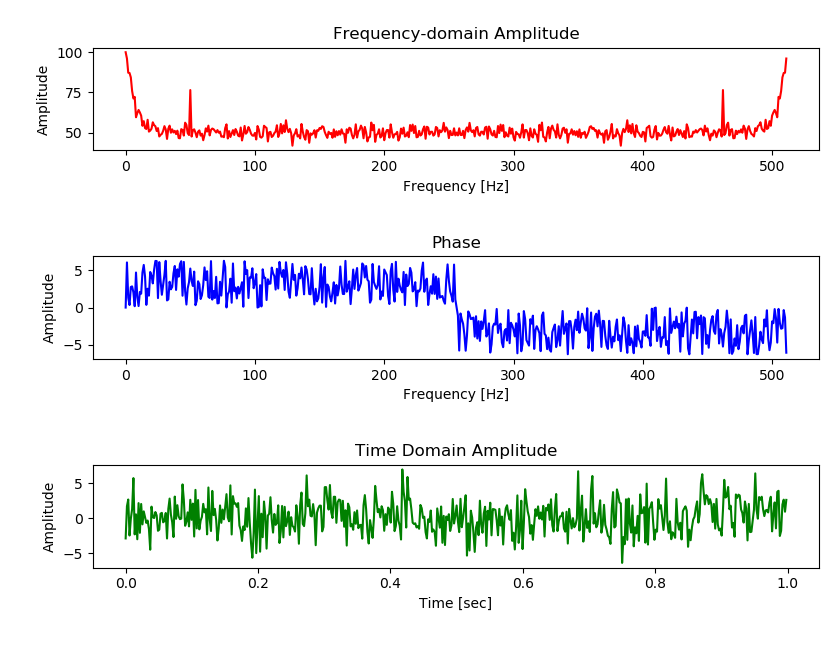
\includegraphics[width=\textwidth]{f2t.png}
	\caption{Example of Generating time-domain series from frequency domain. We have to very careful with symmetry, which requires developers to be familiar with Fourier Transform. }
	\label{fig:f2t}
\end{figure}
\item Create frequency-domain signal series\\
Create plural frequency-domain signal series based on the last step. 
\item Apply Inverse Discrete Fourier Transform\\
After applying inverse Discrete Fourier Transform, we would obtain time-domain signal series. 
\end{enumerate}
%----------------------------------------------------------------------------------------
%	 Excess Power Analysis
%----------------------------------------------------------------------------------------
\chapter{Excess Power Analysis}
\section{Intro}
We obtain the `power' density over frequency after Fourier Transform. If we repeat Fourier Transform over time, we will finally obtain `power' density over both frequency and time, which is called Excess Power Analysis here. 
%From my point of view, this should be addressed as `Power Analysis' without `Excess'. `Excess' refers to the excessive power above the background, which indicates something abnormal or exotic. We will focus on it in the next chapter.\\
\section{Algorithm}
\subsection{Brief Description}
The key point of Excess Power Analysis is Fourier Transform. Actually we deploy Welch’s method instead of classic Fourier Transform. The advantages of Welch’s method are explained in ???(to be written). Anyway, Welch’s method return the power density over frequency. 
We don't care the power density over the entire measurement period. So we slice the data into short segments(like 10s long) first and then apply Welch’s method in each segment. After some further whitening method, we would eventually get the spectrum of `power' density over frequency and time. \\
The process steps are summarized as follows. 
\begin{enumerate}
\item Input necessary parameters
\item Slice data into short segments
\item Apply Welch’s method in each segment 
\item Whiten Power Density Spectrum
\item Draw the spectrum
\end{enumerate}
\subsection{Detailed Description}
\begin{enumerate}
\item Input necessary parameters\\
Parameters for each step will be addressed in the following steps. 
\item Slice data into short segments
\begin{figure}[ht]
	\centering
	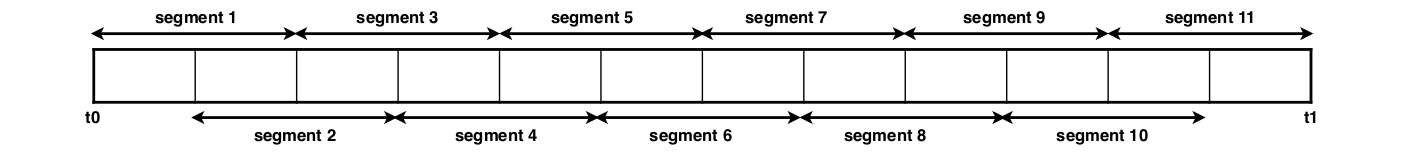
\includegraphics[width=\textwidth]{segments.png}
	\caption{Create overlapping segments in signal series with constant length}
	\label{fig:segments}
\end{figure}\\
\textbf{Segment length} and \textbf{segment stride} are two parameters necessary in this step. For example, we can choose a constant value for segment length like displayed in Fig \ref{fig:segments}.\\
Since we will apply Welch’s method in the next step, data points locating in different positions of the segment would probably not be treated equally, which is caused by windowing procedure in Welch’s method (please refer to windowing or window functions on wiki or other sources if you don't understand). Dishonestly speaking, we have received protest from World Data Right Protection Association (to be founded up). They claimed that every data point should be evenly given the weight to fulfill their value. Under such imaginary pressure, we decided to choose overlapping segments. 
As you can see in the Fig \ref{fig:segments}, segment 1 and segment 2 overlap each other by half of the segment length. The value of it is called segment stride. The data locating near the edge of segment 1 are now near the middle of segment 2. You can choose even large value of segment stride to obtain finer result. \\
To be noticed: As far as I know, nobody limits the value of segment length or stride. In theory, you can choose any size you want. Although constant length is easy to handle, it sometimes has huge problems and result in ugly spectrum or figure. Of course you can choose inconstant values when you have proper reasons.
\item Apply Welch’s method in each segment 
\begin{figure}[ht]
	\centering
	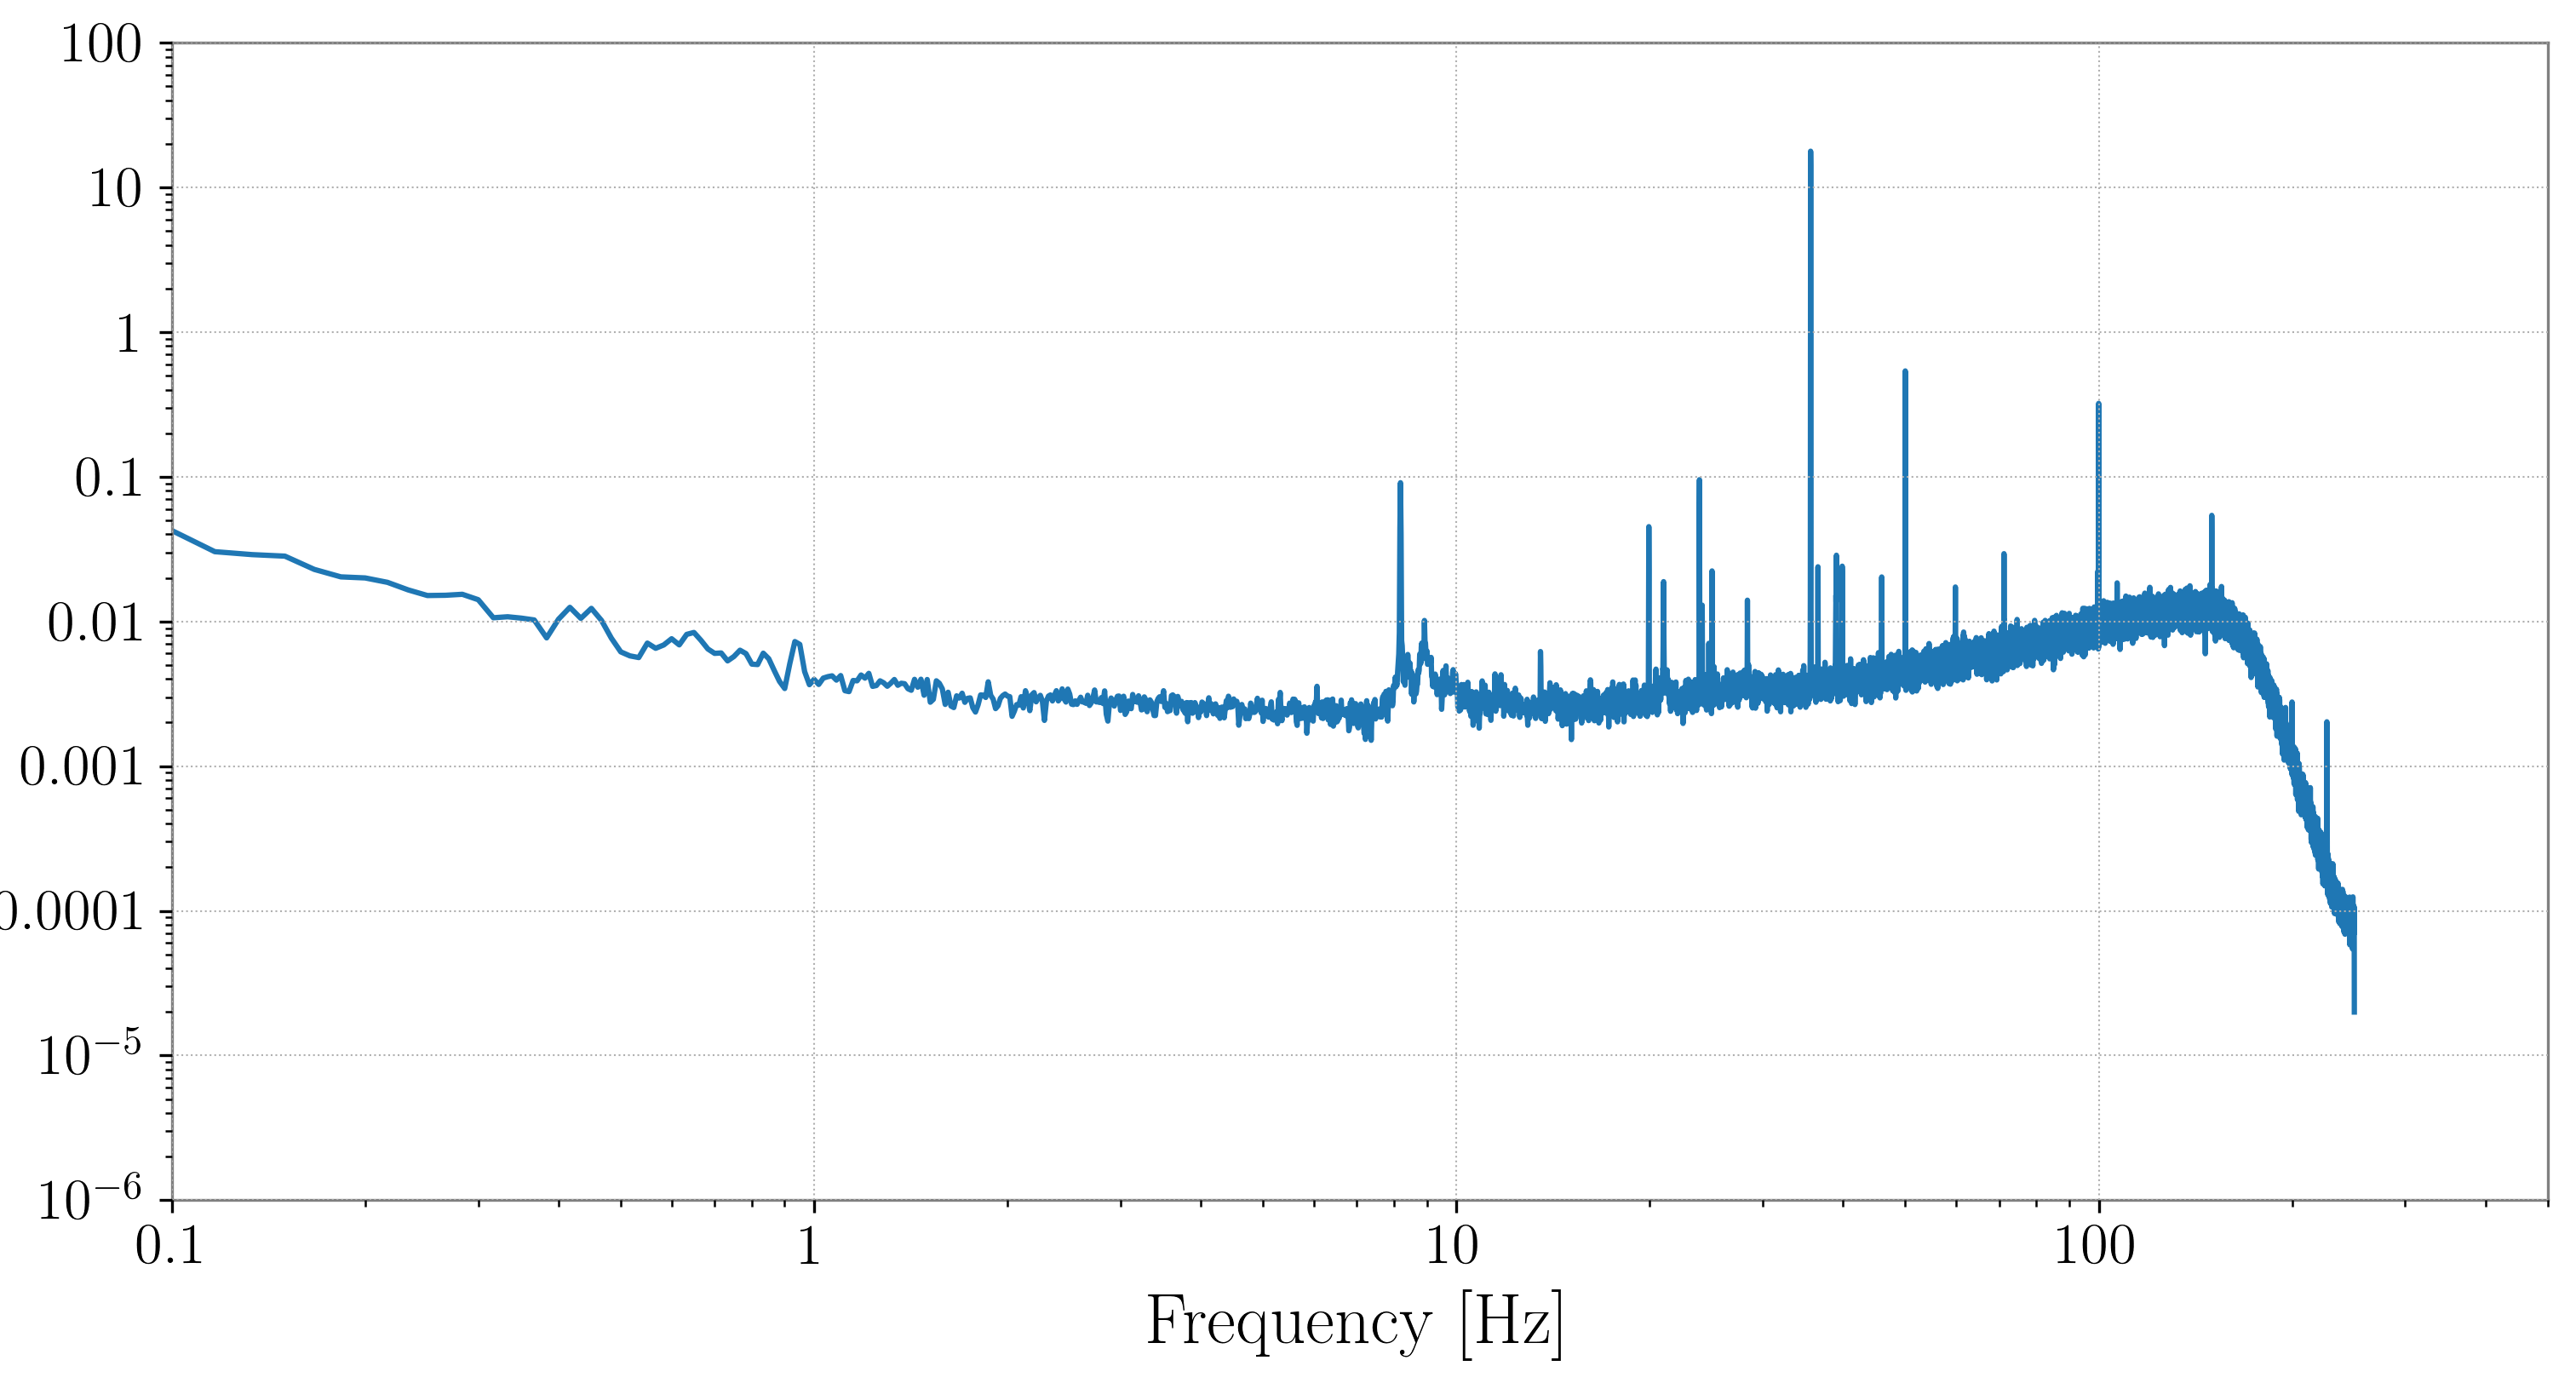
\includegraphics[width=\textwidth]{psd.png}
	\caption{Power Spectral Density (PSD) Example}
	\label{fig:psd}
\end{figure}\\
There are several parameters for Welch's method which are introduced in chapter2(to be written).\\
We apply Welch’s method in each segment. The result of Welch's method, Power Spectral Density (PSD), is displayed in Fig \ref{fig:psd}. The amplitude indicates the 'power' at a certain frequency. You can make a 3D spectrum as shown in Fig \ref{fig:pa}, where the x axis is time and y axis is frequency, while z axis is the amplitude of `power'. The color indicates the power. We call each small square area a `tile'. 
\begin{figure}[ht]
	\centering
	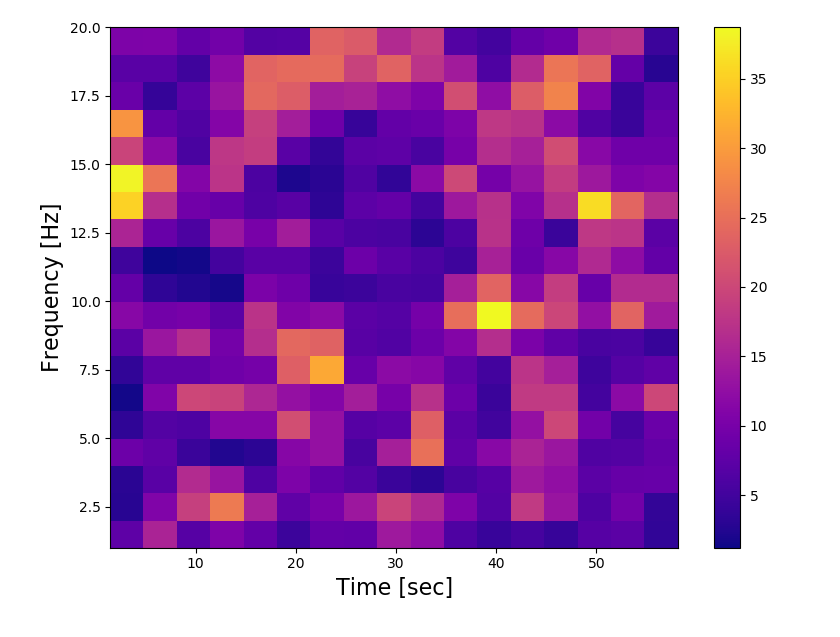
\includegraphics[width=0.8\textwidth]{pa.png}
	\caption{3D spectrum}
	\label{fig:pa}
\end{figure}
\item Whiten Power Density Spectrum\\
The first parameter in this step is \textbf{average method}. We choose a method to whiten the spectrum. After whitening, the spectrum becomes flat where there are merely noise, while it becomes obvious where there's excessive power. \\
Here we introduce Exponentially Moving Average (EMA). Of course there are many other choices. You can choose the most suitable one according to situation. \\
To clear illustrate the problem, let's focus on only one specific frequency band over whole measuring period now. We will repeat the same algorithm for all bands afterwards. \\
It's easy to come up with such an idea to whiten the signal series: We calculate the average value of this band, and make the values of this band be divided by the average. In most cases, the noise amplitudes are close to the average. So we would obtain a whitened signal series with values usually close to $\textbf{1}$. If we find a value far greater than $\textbf{1}$ in the series, it's likely to be a real signal, or so-called excess power. \\
However, actual measurements pose another problem upon this step: The average drifts over time. In experiments, due to the instability of devices, we can whiteness drift over time, like Fig \ref{fig:drift}. 
\begin{figure}[ht]
	\centering
	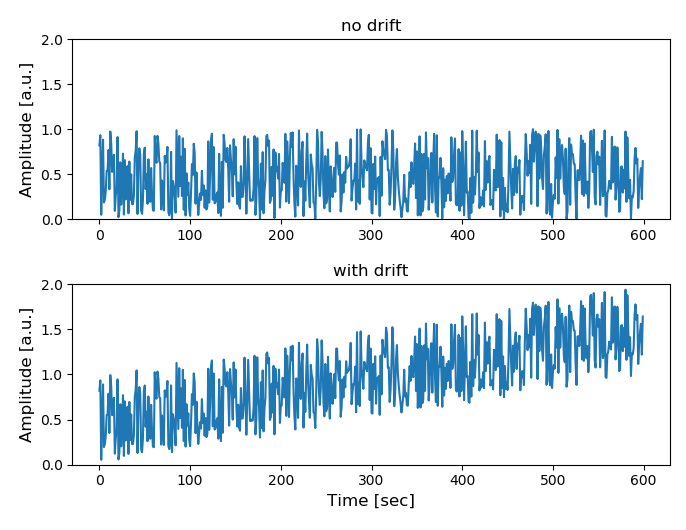
\includegraphics[width=0.8\textwidth]{drift.png}
	\caption{Display of drift over time}
	\label{fig:drift}
\end{figure}\\
Therefore, we believe it's more reasonable to calculate average in a stable period to do the whitening. In other words, when we want to whiten a data point, we should use the average value calculated in a previous period. \\
In addition, we can choose different weights to calculate the average. Normally, we choose exponentially declining over time weights to calculate weighted average. So the weights look like this $e^{-\lambda \Delta t}$ (not normalized), where $\Delta t$ is the time interval between data point and to-be-whitened point. \\
So we have two parameters to be decided in EMA. One is $\lambda$, which is called EMA factor. The other is EMA window length, which decide the range that we calculate the average. 
\item Draw the spectrum\\
Eventually, we draw the 3D spectrum like what's shown in \ref{fig:pa}, but with whitened data this time. 
\end{enumerate}
%\section further thinking on Fourier Transform
%Lorentzian signal and Sine signal
%----------------------------------------------------------------------------------------
%	Single-station Event Identification
%----------------------------------------------------------------------------------------
\chapter{Single-station Event Identification}
\section{Intro}
Finally we are at detection stage. To distinguish signal detection in single- and multi- station situation, \textbf{Identification} is deployed here to emphasize that we are identifying whether a signal is authentic under a certain threshold. While in multi-station detection, \textbf{Locating and Examination} is used to fully describe two unique steps in detection. Single-station signal identification constructs the basis for locating and examining signals in multi-station network.\\
Let’s focus on a single station first.\\
The problem at this stage is simple: We know `power’ distribution over time and frequency from Excess Power Analysis. How to pick up `exotic signals'?\\ %(Please always bare it in mind that, we are playing a game of probability. )
\section{Algorithm}
\subsection{Brief Description}
We will deal with this in statistical way. The key point is to know the probability density distribution over `power', and therefore choose a threshold for picking up `exotic' signals.
\subsection{Detailed Description}
\begin{enumerate}
\item Choose a Certain Set of Parameter for Excess Power analysis\\
Let’s review on the input parameters in data processing. 
\item[] segment length
\item[] segment stride
\item[] Welch’s method number per segment
\item[] average method: default to `Exponential Moving Average (EMA)'
\item[] EMA factor
\item[] EMA window length\\
Here we introduce two more parameters.
\item[] frequency low-pass
\item[] frequency high-pass\\
In the last chapter, we kept all frequency bands on spectrum. However, real signals often respond in a narrow frequency band. We can focus on only the sensitive band of the excess power analysis result. Figure \ref{fig:Lztest} shows different response in frequency domain after being processed by Welch’s method. 
\begin{figure}[h]
	\centering
	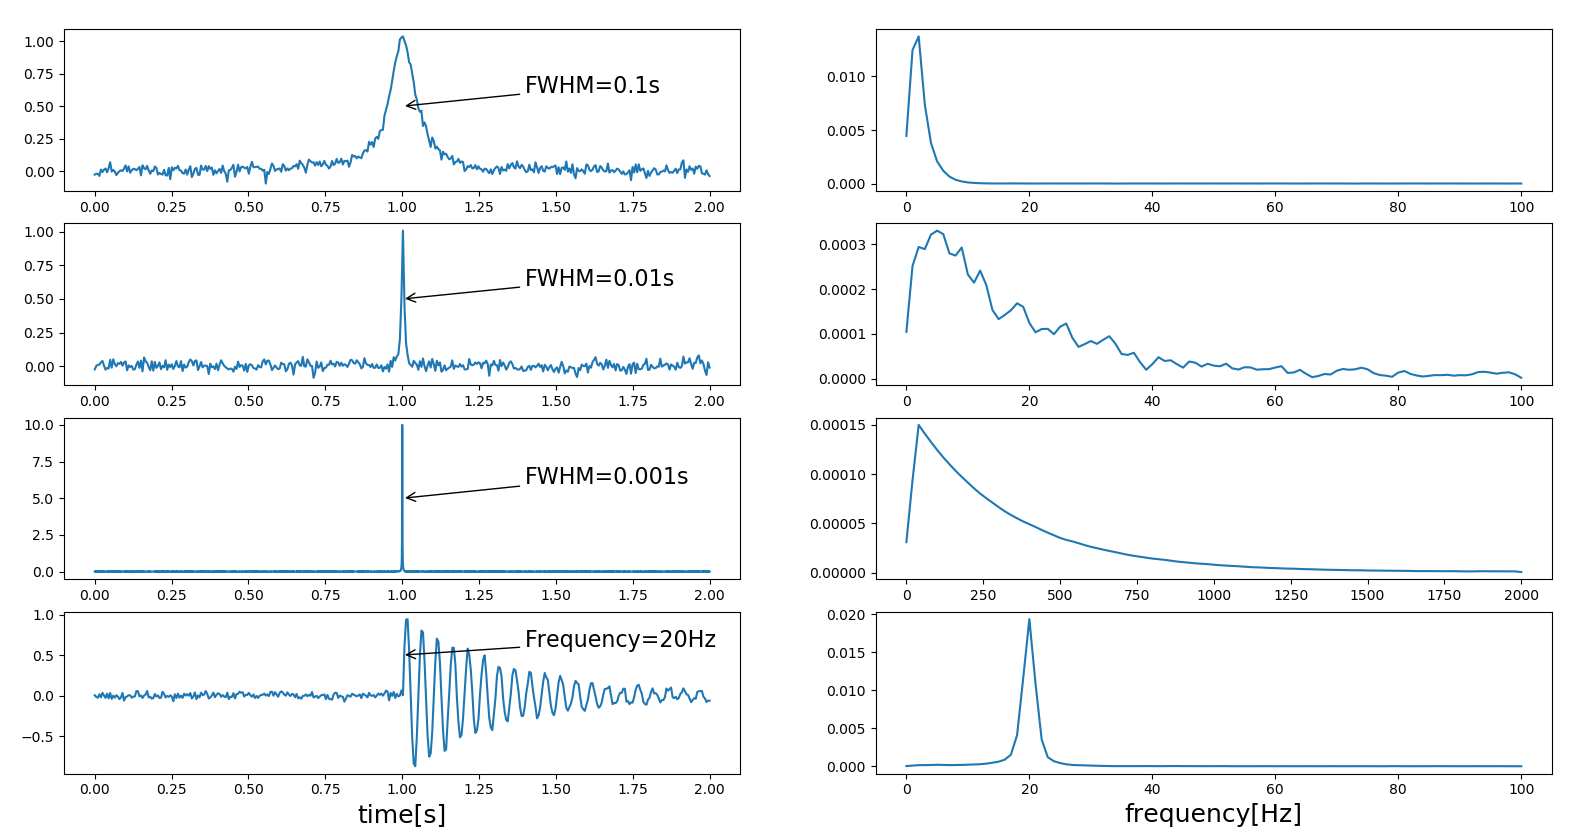
\includegraphics[width=\textwidth]{Lztest.png}
	\caption{Time domain signals (left) and its Welch’s method's result (right)}
\label{fig:Lztest}
\end{figure}\\
People always desire to find the `optimal' parameters for analysis. From my perspective, `optimal' parameters make real signal significant. For example, if you want to search for a Lorentzian signal, of which FWHM is 0.1s, Figure \ref{fig:Lztest} tells you that you'd better focus on frequency from 0 Hz to 5Hz, where its response in frequency domain is at its maximum. \\
There should be a set of `optimal' parameters for analysis under noise with certain characteristics, and signal response to `exotic' physic in a specific sensor. But generally speaking, there's no conclusion which can figure out a general rule for deciding `optimal' parameters. 
Further details on `optimal' parameters will be addressed later in Chapter \ref{ch:MultiStat}. \\
Let's assume that we have known the `optimal' parameters, and move on to the next step. 
\item Creating Background Reference\\
As long as we know the characteristics of the noise, we can simulate it and apply excess power analysis. After statistic methods, we will get the probability density distribution over `power' of noise. This distribution would be the reference to set threshold for `exotic'. We will know how likely it is for us to find a noise signal with certain amplitude in a specific sensor. If we find very rare, it would probably be an `exotic' signal that we are waiting for. 
\end{enumerate}

%\subsection{Find Optimal Parameters for Excess Power Analysis}

%\subsection{Reconstruct Original Signals from Result}
%\textbf{\Large to be completed}

%----------------------------------------------------------------------------------------
%	Multi-station Event Locating and Examination
%----------------------------------------------------------------------------------------
\chapter{Multi-station Event Locating and Examination}\label{ch:MultiStat}

\section{Intro}
Thanks to the construction of global network, we have the confidence in discovering or denying exotic physics. LIGO earned a Nobel Prize with only two stations. The error rate decreases exponentially with the number of stations, so I think we can expect three or even more prizes coming soon.
\section{Assumptions}
Let's take Earth as the reference system. \\%In fact, we have to assume that 
Below are listed some commonly used assumptions. Of course we can revise or even abandon these assumptions when necessary.
\edef\oldassumption{\the\numexpr\value{assumption}+1}
\setcounter{assumption}{0}
\renewcommand{\theassumption}{\oldassumption.\alph{assumption}}
\begin{assumption}[Plane Wave Like]\label{as:PlaneWaveLike}%\label{as:1}
	The perturbation from 'exotic physic' can be described as a plane wave like impact.
\end{assumption}
\begin{assumption}[Constant Velocity]\label{as:ConstantVelocity}%\label{as:1}
	The velocity of perturbation is constant.
\end{assumption}%\let\theassumption\origtheassumption
\noindent Assumption \ref{as:PlaneWaveLike} and \ref{as:ConstantVelocity} decide the distance and time interval of signals between stations. \\
In reality, the perturbation is not likely to be perfect plane wave. Thinking in common sense, there can't be a kind of matter which interacts with the environment while keeping itself unchanged. So the key point is, to which extent does this 'exotic' change after interacting with atoms? We have to assume that the change on the perturbation can be ignored from human’s or Earth’s perspective. Otherwise Assumption \ref{as:PlaneWaveLike} and \ref{as:ConstantVelocity} would be in contradiction with themselves. \\
Two more assumptions are also necessary. 
\edef\oldassumption{\the\numexpr\value{assumption}+1}
\setcounter{assumption}{0}
\renewcommand{\theassumption}{\oldassumption.\alph{assumption}}
\begin{assumption}[Cosine Amplitude]\label{as:CosineAmplitude}
	The amplitude of the signal is proportional to the projection of the plane wave's direction on sensor's sensitive axis.
\end{assumption}
\begin{assumption}[Linear Combination]\label{as:LinearCombination}
	The amplitude of the signal is the linear combination of 'exotic' and others.
\end{assumption}
\noindent Assumption \ref{as:CosineAmplitude} and \ref{as:LinearCombination} decide the amplitude of the signals. Of course we can make more complicated relation than linear and test them by adding several new functions in the program. \\
These rational assumptions are not necessarily true, especially when we are looking for `exotic'. We are just carrying on research under these assumptions for now. \\
\section{Algorithm}
\subsection{Brief Desciption}
From now on, we will be looking for the trace of a perturbation or so-called event in all stations.\\ 
%The following algorithm is the one I realized in program. Obviously, it’s not the only way to discover events. I will provide one more idea later in this section. \\
%When in simulation, we get a straightforward method to locate and examine events.\\

\subsection{Detailed Description}

\begin{enumerate} % [noitemsep] removes whitespace between the items for a compact look
\item Basics\\
To address the problem clearly, we will begin to dicuss in spherical coordinates frame. \\
\begin{figure}[h]
	\begin{center}
	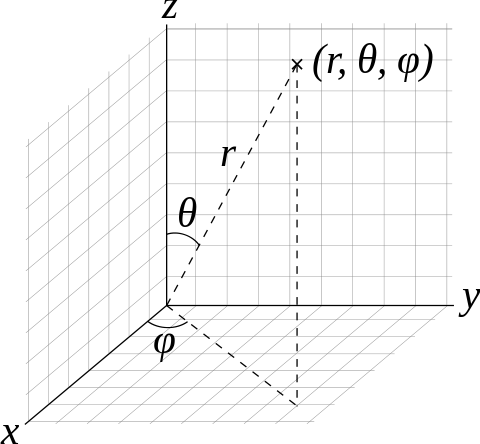
\includegraphics[width=0.4\textwidth]{spherical_frame.png}
	\end{center}
	\caption{Spherical coordinates($r$, $\theta$,$\varphi$). From wiki}
\end{figure}\\
According to Assumption \ref{as:PlaneWaveLike} and \ref{as:ConstantVelocity}, as long as we know the \textbf{locations of all the stations} on Earth, and assume the velocity as $\vec{v}$ (constant), it’s simple to calculate \textbf{time intervals} of signals between stations caused by the same event. The calculation formulas will be illustrated later in realiziation section.
\item Generate reference\\
Let's do some exercises first. Choose directions as shown in Figure \ref{fig:directions}. 
\begin{figure}[htbp]
\centering
\subfigure[directions in vector form]{
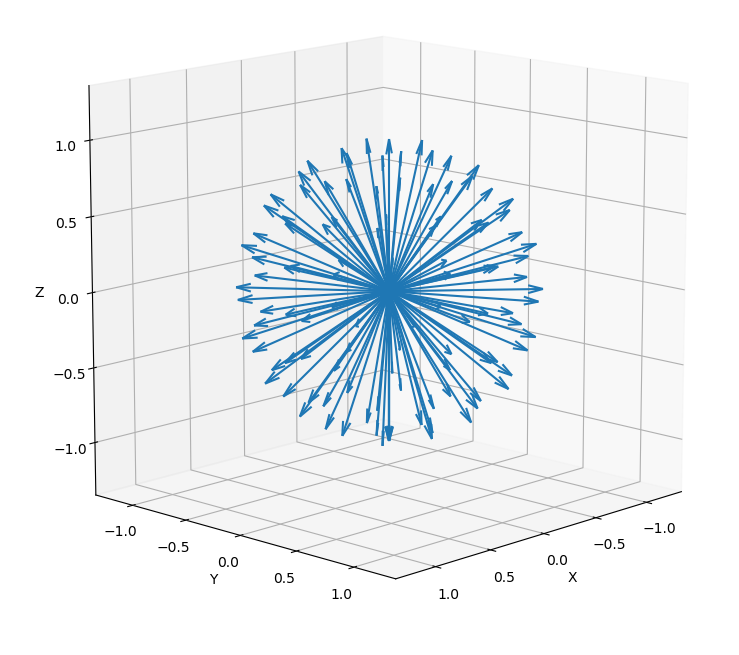
\includegraphics[width=2.7in]{vectors.png}
}
\quad
\subfigure[directions in scatter form]{
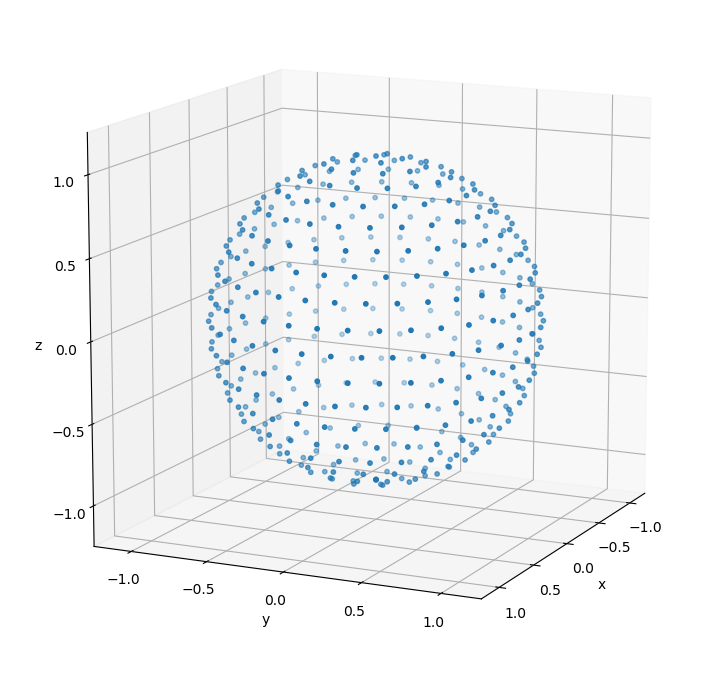
\includegraphics[width=2.7in]{scatters.png}
}
\caption{Directions. Vectors indicate the directions, while making it hard to recognize directions when there's too many. Scatters indicate the directions in a more fresh way. }
\label{fig:directions}
\end{figure}
Since we know the \textbf{locations of all the stations} on Earth, we can calculate time intervals between stations in all these different directions. \\
What we care about is the relative time interval between stations, so we can choose the time as \textbf{0} when one station first receive the perturbation. And by choosing a proper speed, we can always make it \textbf{1} the time when the last station receive the perturbation .\\
Then we save the directions and its time intervals as file. Basically, this is what can perform as reference for time intervals.
\item Locate Events\\
After generating the reference, we can get started to seek events. \\
We can infer from Assumption \ref{as:PlaneWaveLike} that, one perturbation would leave one signal in a sensor. By picking up one signal from one stations, we get a set of signals. We can call this \textbf{potential event}, which means it could arise from the same perturbation, or merely noise, or mixture of them two. \\
Let's determine the problem we are coping with now. We have this \textbf{potential event}, and we know the time intervals between signals in this event, so we are trying to locate the direction of the perturbation which caused this \textbf{potential event}. \\
Since we are looing for its direction, we can let alone the speed of the perturbation at present. We repeat the linear transform to transform the time intervals into [0, 1], which means the time is set as \textbf{0} when the first station received the perturbation, and time is set as \textbf{1} when the last station received the perturbation. \\
We can look into the reference, and try to find a match between time intervals in the \textbf{potential event} and in reference. Of course there would not be a perfect match. But there could be some approximate match, which indicates a \textbf{real event}. There also could be no approximate match, which indicates a \textbf{fake event}.\\
I realized the following test in the program: Input the direction of a perturbation, and obtain a set of time intervals, which can be defined as `to-be-located intervals'. Compare it with reference, and pick up three directions in the reference which match the `to-be-located intervals' best. We can see the result in Figure \ref{fig:test}. We can further locate the direction of the perturbation by generating a finer reference.
\begin{figure}[h]
	\begin{center}
	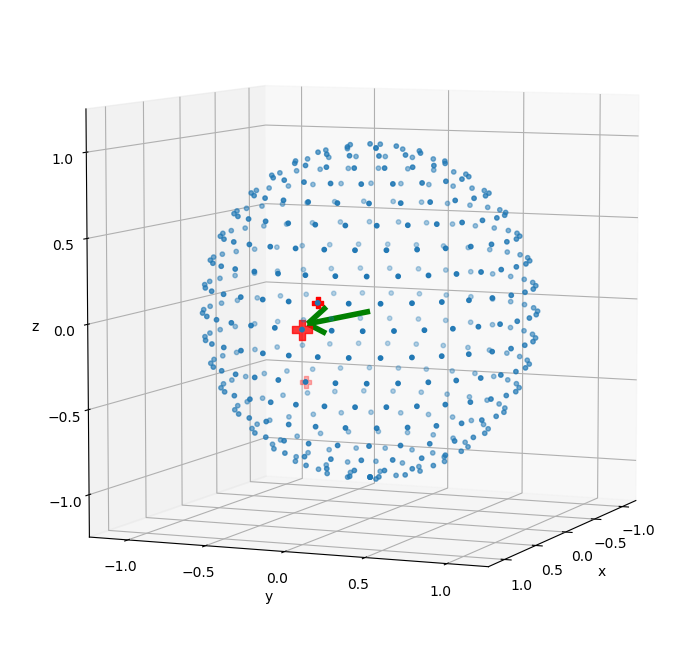
\includegraphics[width=0.9\textwidth]{locating.png}
	\end{center}
	\caption{The green vector is real direction of perturbation. Red dots indicate three best-match directions in the reference which match the real direction well.}
\label{fig:test}
\end{figure}
\item Examine the Result\\
As mentioned before, we are play the game of probability. We have to calculate the confidence or uncertainty of the perturbation direction. \\
Additionally, we have to take signal amplitude and perturbation speed into examination. \\
Sadly, there’s no conclusion to tell us how to calculate the confidence based on these factors. This part is to be completed.
\item Further Thinking\\
Now we’ve got a big network around the world. I believe that perturbations coming from different directions will have their unique sets of time intervals, which is the ‘fingerprint’ of the direction. However, this is not necessarily true, especially when few stations response to the event. For example, when we get only three station, we can only tell the direction in the plane constructed by the stations.\\
There’s one more thing to be cautious with: we can never find the direction perfectly in nature for two reasons. Firstly, the reference is created via interpolation in directions. Secondly, when in excess power analysis, we divide the signal series into segments. We have no means to locate the signal accurately in this segment. The second reason is the fundamental reason. Even with perfect device and precise measurement, it’s impossible to locate the signal. To deal with this, we could choose a smaller segment length in excess power analysis at the expense of frequency resolution. Or do finer analysis in excess power analysis at the expense of huge calculations and our brain cells.\\
There are more factors in preventing as from find the perfect match, like the uncertainty in time-sync, flaws in previous assumptions and so on.\\
\end{enumerate}
%\subsection{Drawbacks}
%You may have already realized the disadvantages of this algorithm.\\
%The calculation amount increases quickly with the number of ‘exotic’ signals selected from each stations. For instance, there’s only one combination if we pick up only one signal from each station. But there would be $2^{n}$ combinations if we take 2 signals from n stations.\\
%What’s worse, it happens that not every station responses apparently to the event because of the sensitive axis. We may not pick up all the signals caused by one event. Therefore it’s more acceptable not to locate the event by examining the combination of ‘exotic’ signals from all stations. \\
%\subsection{Modifications}
%\textbf{\Large more to be written here}

%\subsection{Another Algorithm in Locating and Examination}
%Since I didn't realize this algorithm in program, I will just intruduce this method briefly for the time being. \\
%Instead of comparing the set of picked-up signals with reference, we take time intervals in the reference to scan the signal series. \\
%Let me take an example to illustrate it. 

%

\subsection{Optimal Parameters for Excess Power Analysis}
You will obtain different result with different sets of parameters. When the real signals are weak (SNR$\sim$1), good sets of parameters will accurately make the segments containing real signals obvious, while bad sets make the real signal less apparent. \\
There can’t be a more stupid idea than mine: try all sets of parameters and pick up the best one. However, I don’t recommend any clever way. There’s no conclusion in deciding or calculating the best choice. Also, I don’t recommend you look for any conclusion or formula in choosing parameters. I tried to find some ‘trends’ with simulation in deciding the optimal parameters. I did find some limitations for parameters which are shown at the end of this subsection. But generally speaking, there’s no definite conclusion. Considering the quantity of all these parameters, it’s certainly time-consuming to seek a easy conclusion. By the way, I feel doubtful about the existence of such ‘conclusion’. \\
Let’s review on the input parameters in data processing.
\begin{enumerate}
\item[] segment length
\item[] segment stride
\item[] Welch’s method number per segment
\item[] average method: default to ‘Exponential Moving Average (EMA)’
\item[] EMA factor
\item[] EMA window length
\item[] frequency low-pass
\item[] frequency high-pass
\end{enumerate}
Let me illustrate the simulation with an example.
\begin{enumerate}
\item Generate Signal series\\
Considering the random noise, we can generate many signal series.
\item Choose different sets of parameters\\
We choose different sets of parameters. 
\item Simulation test\\
We test each set of parameters with each signal series.
\item Select the optimal set of parameters\\
Finally, under some criteria, we pick up the best set of parameters for the identification in a specific sensor. 
\end{enumerate}
Though there’s no definite conclusion in deciding parameters, there are some tips or precautions just for reference. 
\begin{enumerate}
\item Segment length\\
Large segment length could be a trouble in locating the signal in time domain. Imagine that we set length to 1000s, then it’s impossible to locate the signal at 10s scale. Additionally, we would get one more problem. More ‘power’ would accumulate in a larger segment, which makes the signal less apparent. What’s worse, the sensors may not be stable over a long time.
Little segment length will result in bad frequency resolution. With a certain sampling rate, a smaller segment contains less data point, which limits the resolution in frequency. We can set the lower limit for segment length according to the desired resolution.
\item EMA factor\\
Greater factor would decrease the influence of more previous segments. Imagine that we set factor to 100, and segment stride to 2s. The weights(not normalized) of the previous segments would be 1, exp(-100), exp(-200)... so that only the closest one segment contributes to the whitening, which would probably increase the variance (just ‘probably’).
\item EMA window length\\
We have less confidence to choose a small window to whiten the signal series.
Large window usually leads to heavy burden for computing. Also, considering the stability of the sensors, it’s not reasonable to choosing an extremely large window.
\end{enumerate}
%----------------------------------------------------------------------------------------
%	BIBLIOGRAPHY
%----------------------------------------------------------------------------------------
%\renewcommand{\refname}{\spacedlowsmallcaps{References}} % For modifying the bibliography heading

%\bibliographystyle{unsrt}

%\bibliography{sample.bib} % The file containing the bibliography

%----------------------------------------------------------------------------------------
\end{document}